\documentclass[11pt,a4paper]{article}

% ==============================================================================
% PACKAGES & SYSTEM SETUP
% ==============================================================================
\usepackage[T1]{fontenc}
\usepackage{mathpazo}          % Palatino font for mathematical typography
\usepackage[scaled=0.92]{helvet}% Clean sans-serif for headers and titles
\usepackage{inconsolata}        % Monospace font for code

\usepackage[margin=0.6in, top=0.65in, bottom=0.65in]{geometry}
\usepackage{amsmath, amssymb, amsthm}
\usepackage{mathtools}
\usepackage{booktabs}
\usepackage{colortbl}
\usepackage{tabularx}
\usepackage{enumitem}
\usepackage{graphicx}
\usepackage[table]{xcolor}
\usepackage{fancyhdr}
\usepackage{lastpage}
\usepackage{microtype}
\usepackage{fontawesome5}

\usepackage[most]{tcolorbox}
\usepackage{tikz}
\usepackage{pgfplots}
\pgfplotsset{compat=1.18}
\usetikzlibrary{positioning, calc, shapes.geometric, backgrounds, patterns}

% ==============================================================================
% COLOR PALETTE (Modern Slate & Muted Teal)
% ==============================================================================
\definecolor{NavyPrimary}{HTML}{1E293B}   % Deep Slate Navy
\definecolor{TealAccent}{HTML}{0D9488}    % Muted Modern Teal
\definecolor{SoftBg}{HTML}{F8FAFC}        % Light Canvas Gray
\definecolor{BorderGray}{HTML}{CBD5E1}    % Clean Border Gray
\definecolor{CharcoalText}{HTML}{334155}  % High-contrast Body Text
\definecolor{CodeBg}{HTML}{F1F5F9}        % Light Code Background
\definecolor{AlertAmber}{HTML}{B45309}    % Muted Amber Callout

\usepackage[hidelinks, colorlinks=true, linkcolor=TealAccent, citecolor=TealAccent, urlcolor=TealAccent]{hyperref}

% ==============================================================================
% PAGE HEADER & FOOTER SETUP
% ==============================================================================
\pagestyle{fancy}
\fancyhf{}
\renewcommand{\headrulewidth}{0.4pt}
\renewcommand{\footrulewidth}{0.4pt}
\headsep = 10pt

\lhead{\small\sffamily\bfseries\color{NavyPrimary} ECON 4120: Empirical Macroeconomics \& Econometrics}
\rhead{\small\sffamily\color{CharcoalText} Problem Set 3 --- Spring 2026}
\lfoot{\small\sffamily\color{CharcoalText}\faUniversity\ Department of Economics}
\cfoot{}
\rfoot{\small\sffamily\color{CharcoalText} Page \thepage\ of \pageref{LastPage}}

% ==============================================================================
% CUSTOM TCOLORBOX STYLES
% ==============================================================================
\tcbset{
    problembox/.style={
        enhanced,
        colback=SoftBg,
        colframe=NavyPrimary,
        boxrule=0.8pt,
        arc=3pt,
        left=7pt, right=7pt, top=4pt, bottom=4pt,
        fonttitle=\sffamily\bfseries,
        coltitle=white,
        attach boxed title to top left={xshift=7pt, yshift=-7pt},
        boxed title style={
            colback=NavyPrimary,
            colframe=NavyPrimary,
            arc=2.5pt,
            outer arc=2.5pt,
            boxsep=2pt
        }
    },
    solutionbox/.style={
        enhanced,
        colback=white,
        colframe=TealAccent,
        boxrule=0.5pt,
        arc=2.5pt,
        left=7pt, right=7pt, top=4pt, bottom=4pt,
        borderline west={2.5pt}{0pt}{TealAccent}
    },
    infobox/.style={
        enhanced,
        colback=SoftBg,
        colframe=BorderGray,
        boxrule=0.5pt,
        arc=2.5pt,
        left=7pt, right=7pt, top=4pt, bottom=4pt,
        borderline west={2.5pt}{0pt}{NavyPrimary}
    },
    codebox/.style={
        enhanced,
        colback=CodeBg,
        colframe=BorderGray,
        boxrule=0.5pt,
        arc=2pt,
        fontupper=\ttfamily\small,
        left=7pt, right=7pt, top=4pt, bottom=4pt
    }
}

% Custom Subproblem Command
\newcounter{subprob}[section]
\newcommand{\subproblem}[1]{%
    \par\vspace{2pt}\noindent%
    \refstepcounter{subprob}%
    \textbf{\sffamily\color{NavyPrimary}(\alph{subprob})} #1\par\vspace{1pt}%
}

% Redefine Section Style
\makeatletter
\renewcommand{\section}{\@startsection{section}{1}{0pt}%
    {-1.2ex plus -0.3ex minus -.1ex}%
    {0.5ex plus .1ex}%
    {\normalfont\large\sffamily\bfseries\color{NavyPrimary}}}
\makeatother

% ==============================================================================
% DOCUMENT CONTENT
% ==============================================================================
\begin{document}

% ------------------------------------------------------------------------------
% ASSIGNMENT HEADER BANNER
% ------------------------------------------------------------------------------
\begin{tcolorbox}[
    enhanced,
    colback=NavyPrimary,
    coltext=white,
    arc=3.5pt,
    boxrule=0pt,
    left=10pt, right=10pt, top=6pt, bottom=6pt
]
\begin{minipage}[c]{0.54\linewidth}
    {\Large\sffamily\bfseries Advanced Econometrics \& Dynamic Theory}\\[2pt]
    {\large\sffamily\color{TealAccent!40} Problem Set 3: Causal Inference \& Dynamic Optimization}\\[3pt]
    {\scriptsize\sffamily\color{white!85}\faChalkboardTeacher\ Instructor: Prof. Aris Thorne \quad|\quad \faGraduationCap\ Department of Economics}
\end{minipage}%
\begin{minipage}[c]{0.44\linewidth}
    \raggedleft
    \scriptsize\sffamily
    \begin{tabular}{ll}
        \textbf{Course Code:} & ECON 4120 / 6120 \\
        \textbf{Date Issued:} & March 14, 2026 \\
        \textbf{Submission Due:} & March 28, 2026 (23:59 EST) \\
        \textbf{Target Audience:} & Senior Undergrad / Graduate
    \end{tabular}
\end{minipage}
\end{tcolorbox}

\vspace{1pt}

% Student Metadata Submission Block
\begin{tcolorbox}[infobox]
    \scriptsize\sffamily
    \begin{minipage}[c]{0.48\linewidth}
        \textbf{Student Name:} \underline{\hspace{4.2cm}}
    \end{minipage}%
    \begin{minipage}[c]{0.52\linewidth}
        \raggedleft
        \textbf{Student ID / Matriculation:} \underline{\hspace{3.4cm}}
    \end{minipage}
    \par\vspace{2pt}
    \begin{minipage}[c]{0.74\linewidth}
        \color{CharcoalText}\faInfoCircle\ \textit{Instructions: Show all derivation steps for analytical questions. Attach executable R scripts for empirical sections.}
    \end{minipage}%
    \begin{minipage}[c]{0.26\linewidth}
        \raggedleft
        \textbf{Score / Total:} \framebox[1.6cm][c]{\strut \quad / 100}
    \end{minipage}
\end{tcolorbox}

\vspace{2pt}

% ==============================================================================
% PAGE 1 - PART I: THEORETICAL MACROECONOMICS & DYNAMIC OPTIMIZATION
% ==============================================================================
\section{Part I: Intertemporal Choice \& Liquidity Constraints}

\begin{tcolorbox}[problembox, title={Problem 1: Household Consumption Smoothing under Borrowing Limits (25 Points)}]
Consider a two-period consumption problem. A household receives endowment $y_1 > 0$ in Period 1 and $y_2 > 0$ in Period 2, maximizing CRRA utility $U(c_1, c_2) = \frac{c_1^{1-\gamma} - 1}{1-\gamma} + \beta \left( \frac{c_2^{1-\gamma} - 1}{1-\gamma} \right)$ with $\gamma > 0, \gamma \neq 1, \beta \in (0, 1)$, subject to interest rate $r > 0$ and borrowing limit $c_1 \le y_1$.
\end{tcolorbox}

\setcounter{subprob}{0}

\subproblem{Formulate the constrained optimization problem using the Lagrangian method and derive the modified Euler equation.}

\begin{tcolorbox}[solutionbox]
\textbf{\sffamily\color{TealAccent} Solution:}
Writing the Lagrangian with borrowing constraint multiplier $\lambda \ge 0$:
\[
    \mathcal{L} = \frac{c_1^{1-\gamma} - 1}{1-\gamma} + \beta \left( \frac{c_2^{1-\gamma} - 1}{1-\gamma} \right) + \mu \left[ y_1 + \frac{y_2}{1+r} - c_1 - \frac{c_2}{1+r} \right] + \lambda (y_1 - c_1)
\]
First-order conditions $\frac{\partial \mathcal{L}}{\partial c_1} = c_1^{-\gamma} - \mu - \lambda = 0$ and $\frac{\partial \mathcal{L}}{\partial c_2} = \beta c_2^{-\gamma} - \frac{\mu}{1+r} = 0$ yield the modified Euler Equation:
\begin{equation}
    c_1^{-\gamma} = \beta (1+r) c_2^{-\gamma} + \lambda
\end{equation}
Complementary slackness requires $\lambda \ge 0$, $(y_1 - c_1) \ge 0$, and $\lambda (y_1 - c_1) = 0$. When the borrowing limit binds ($\lambda > 0$), $c_1^* = y_1$, $c_2^* = y_2$, and marginal utility satisfies $c_1^{-\gamma} > \beta(1+r)c_2^{-\gamma}$.
\end{tcolorbox}

\subproblem{Graphically illustrate optimal allocation $(c_1^*, c_2^*)$ under (i) Unconstrained regime ($\lambda = 0$) and (ii) Binding constraint ($\lambda > 0$).}

\begin{figure}[htbp]
\centering
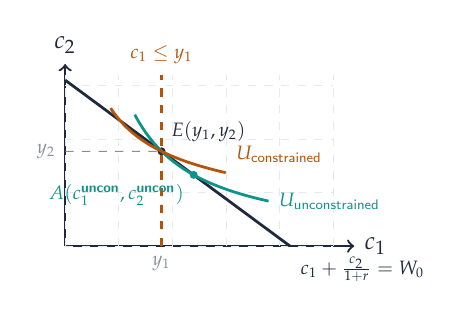
\begin{tikzpicture}[scale=0.68]
    \draw[->, thick, color=NavyPrimary] (0,0) -- (5.4,0) node[right, font=\sffamily\small] {$c_1$};
    \draw[->, thick, color=NavyPrimary] (0,0) -- (0,3.4) node[above, font=\sffamily\small] {$c_2$};
    \draw[help lines, color=BorderGray!50, dashed] (0,0) grid (5.0,3.2);
    
    \draw[line width=1.0pt, color=NavyPrimary] (0,3.1) -- (4.2,0) node[below right, font=\sffamily\scriptsize] {$c_1 + \frac{c_2}{1+r} = W_0$};
    
    \coordinate (E) at (1.8, 1.77);
    \filldraw[color=NavyPrimary] (E) circle (1.8pt) node[above right, font=\sffamily\scriptsize\bfseries] {$E(y_1, y_2)$};
    \draw[dashed, color=CharcoalText!60] (1.8,0) node[below, font=\sffamily\scriptsize] {$y_1$} -- (E) -- (0,1.77) node[left, font=\sffamily\scriptsize] {$y_2$};
    \draw[line width=1.1pt, color=AlertAmber, dashed] (1.8,0) -- (1.8,3.2) node[above, font=\sffamily\scriptsize] {$c_1 \le y_1$};
    
    \coordinate (A) at (2.4, 1.33);
    \draw[line width=1.0pt, color=TealAccent, domain=1.3:3.8, samples=80] 
        plot (\x, {1.33*2.4/\x}) node[right, font=\sffamily\scriptsize] {$U_{\text{unconstrained}}$};
    \filldraw[color=TealAccent] (A) circle (1.8pt) node[below left, font=\sffamily\scriptsize\bfseries] {$A(c_1^{\text{uncon}}, c_2^{\text{uncon}})$};
    
    \draw[line width=1.0pt, color=AlertAmber, domain=0.85:3.0, samples=80] 
        plot (\x, {1.77*sqrt(1.8/\x)}) node[above right, font=\sffamily\scriptsize] {$U_{\text{constrained}}$};
\end{tikzpicture}
\caption{\sffamily Intertemporal Consumption Choice under Borrowing Constraints. Low $y_1$ causes unconstrained point $A$ to violate $c_1 \le y_1$, forcing consumption to endowment point $E$.}
\label{fig:intertemporal}
\end{figure}

\clearpage

% ==============================================================================
% PAGE 2 - PART II: APPLIED ECONOMETRICS & CAUSAL INFERENCE
% ==============================================================================
\section{Part II: Endogeneity, Instrumental Variables \& 2SLS}

\begin{tcolorbox}[problembox, title={Problem 2: Estimating Skill Returns at Nexa Analytics (35 Points)}]
An econometrician at \textbf{Nexa Analytics} evaluates technical training ($\text{Educ}_i$) on log hourly earnings ($\ln(W_i)$):
\begin{equation}
    \ln(W_i) = \beta_0 + \beta_1 \text{Educ}_i + \beta_2 \text{Exper}_i + u_i
\end{equation}
Unobserved ability ($A_i$) induces endogeneity: $u_i = \gamma A_i + v_i$ with $\text{Cov}(\text{Educ}_i, u_i) > 0$. The instrument $Z_i$ is childhood distance to public university.
\end{tcolorbox}

\setcounter{subprob}{0}

\subproblem{Draw the Causal Directed Acyclic Graph (DAG) for $Z_i$, $\text{Educ}_i$, $\ln(W_i)$, and $A_i$. State key identification conditions.}

\begin{tcolorbox}[solutionbox]
\textbf{\sffamily\color{TealAccent} Identification Analysis \& Causal DAG:}

\begin{center}
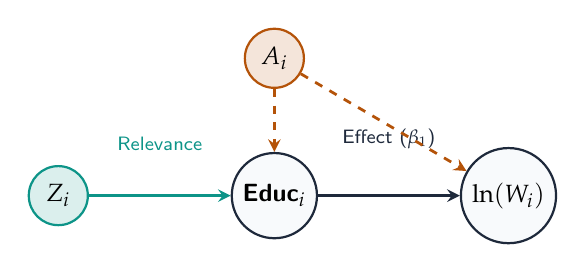
\begin{tikzpicture}[
    node distance=1.1cm and 1.8cm,
    font=\sffamily\small,
    every node/.style={circle, draw=NavyPrimary, fill=SoftBg, inner sep=2.5pt, minimum size=0.75cm, line width=0.8pt},
    arrow/.style={->, >=stealth, line width=1.0pt, color=NavyPrimary},
    dashedarrow/.style={->, >=stealth, line width=1.0pt, color=AlertAmber, dashed}
]
    \node (Z) [fill=TealAccent!15, draw=TealAccent] {\textbf{$Z_i$}};
    \node (X) [right=of Z] {\textbf{$\text{Educ}_i$}};
    \node (Y) [right=of X] {\textbf{$\ln(W_i)$}};
    \node (U) [above=0.8cm of X, fill=AlertAmber!15, draw=AlertAmber] {\textbf{$A_i$}};

    \draw[arrow, color=TealAccent] (Z) -- node[above, draw=none, fill=none] {\scriptsize Relevance} (X);
    \draw[arrow] (X) -- node[above, draw=none, fill=none] {\scriptsize Effect ($\beta_1$)} (Y);
    \draw[dashedarrow] (U) -- (X);
    \draw[dashedarrow] (U) -- (Y);
\end{tikzpicture}
\end{center}

Identification requirements:
\begin{enumerate}[label=\arabic*., topsep=1pt, itemsep=1pt]
    \item \textbf{Relevance:} $\text{Cov}(Z_i, \text{Educ}_i \mid \text{Exper}_i) \neq 0$ (Verified via First-Stage $F > 10$).
    \item \textbf{Exclusion Restriction \& Exogeneity:} $\text{Cov}(Z_i, u_i) = 0$ ($Z_i$ affects wages only through education).
\end{enumerate}
\end{tcolorbox}

\subproblem{Algebraically prove that the 2SLS estimator $\hat{\boldsymbol{\beta}}_{\text{2SLS}}$ is consistent for $\boldsymbol{\beta}$ in matrix notation.}

\begin{tcolorbox}[solutionbox]
\textbf{\sffamily\color{TealAccent} Proof of 2SLS Consistency:}

Let projection matrix $\mathbf{P}_Z = \mathbf{Z}(\mathbf{Z}'\mathbf{Z})^{-1}\mathbf{Z}'$. The 2SLS estimator $\hat{\boldsymbol{\beta}}_{\text{2SLS}} = \left( \mathbf{X}'\mathbf{P}_Z\mathbf{X} \right)^{-1} \mathbf{X}'\mathbf{P}_Z\mathbf{Y}$ expands to:
\begin{equation}
    \hat{\boldsymbol{\beta}}_{\text{2SLS}} - \boldsymbol{\beta} = \left[ \left(\frac{\mathbf{X}'\mathbf{Z}}{N}\right) \left(\frac{\mathbf{Z}'\mathbf{Z}}{N}\right)^{-1} \left(\frac{\mathbf{Z}'\mathbf{X}}{N}\right) \right]^{-1} \left(\frac{\mathbf{X}'\mathbf{Z}}{N}\right) \left(\frac{\mathbf{Z}'\mathbf{Z}}{N}\right)^{-1} \left(\frac{\mathbf{Z}'\mathbf{u}}{N}\right)
\end{equation}
As $N \to \infty$, $\frac{1}{N}\mathbf{Z}'\mathbf{Z} \xrightarrow{p} \boldsymbol{\Sigma}_{ZZ}$ and $\frac{1}{N}\mathbf{Z}'\mathbf{X} \xrightarrow{p} \boldsymbol{\Sigma}_{ZX}$. By Exogeneity, $\frac{1}{N}\mathbf{Z}'\mathbf{u} \xrightarrow{p} \mathbf{0}$. By Slutsky's Theorem:
\[
    \text{plim}_{N \to \infty} \left( \hat{\boldsymbol{\beta}}_{\text{2SLS}} - \boldsymbol{\beta} \right) = \left[ \boldsymbol{\Sigma}_{XZ} \boldsymbol{\Sigma}_{ZZ}^{-1} \boldsymbol{\Sigma}_{ZX} \right]^{-1} \boldsymbol{\Sigma}_{XZ} \boldsymbol{\Sigma}_{ZZ}^{-1} \cdot \mathbf{0} = \mathbf{0} \implies \hat{\boldsymbol{\beta}}_{\text{2SLS}} \xrightarrow{p} \boldsymbol{\beta} \qed
\]
\end{tcolorbox}

\subproblem{Explain the weak instrument problem. What statistic evaluates instrument strength, and what threshold is used?}

\begin{tcolorbox}[solutionbox]
\textbf{\sffamily\color{TealAccent} Weak Instruments \& First-Stage Diagnostics:}

Weak instruments ($\text{Cov}(Z, X) \approx 0$) bias 2SLS toward OLS and invalidate standard test inference. First-Stage effective $F$-statistic evaluates strength: $F = \frac{(\mathbf{R}\hat{\boldsymbol{\pi}})'[\mathbf{R}\widehat{\text{Var}}(\hat{\boldsymbol{\pi}})\mathbf{R}']^{-1}(\mathbf{R}\hat{\boldsymbol{\pi}})}{q}$. Stock-Yogo rule of thumb requires $F > 10$ to ensure 2SLS bias is under 10\% of OLS bias.
\end{tcolorbox}

\clearpage

% ==============================================================================
% PAGE 3 - PART III: EMPIRICAL ANALYSIS & REGRESSION BENCHMARKING
% ==============================================================================
\section{Part III: Panel Econometrics \& Corporate R\&D at Vertex Global}

\begin{tcolorbox}[problembox, title={Problem 3: Panel Data Estimation of Productivity Dynamics (40 Points)}]
Using a balanced panel of 450 industrial units at \textbf{Vertex Global} over $T = 10$ years ($N \times T = 4,500$), we estimate log Total Factor Productivity: $\ln(\text{TFP}_{it}) = \alpha_i + \gamma_t + \beta_1 \text{RD}_{it} + \beta_2 \text{CapLab}_{it} + \beta_3 \text{MarketShare}_{it} + \varepsilon_{it}$.
\end{tcolorbox}

\begin{table}[htbp]
\centering
\caption{\sffamily Panel Regression Results: Determinants of Productivity ($\ln(\text{TFP}_{it})$)}
\label{tab:regression}
\vspace{2pt}
\scriptsize
\begin{tabularx}{\textwidth}{X *{4}{c}}
\toprule
\textbf{Independent Variables} & \textbf{(1) Pooled OLS} & \textbf{(2) Random Effects} & \textbf{(3) Fixed Effects} & \textbf{(4) 2SLS Fixed Effects} \\
\midrule
R\&D Intensity ($\text{RD}_{it}$) & 0.412*** & 0.328*** & 0.215** & 0.284*** \\
 & (0.048) & (0.041) & (0.072) & (0.081) \\
Capital-Labor Ratio & 0.185*** & 0.162*** & 0.118** & 0.124** \\
 & (0.032) & (0.029) & (0.045) & (0.047) \\
Market Share & 0.094** & 0.071* & 0.023 & 0.019 \\
 & (0.031) & (0.033) & (0.041) & (0.043) \\
\midrule
Firm \& Year Fixed Effects & No / Yes & RE / Yes & Yes / Yes & Yes / Yes \\
Instrument & None & None & None & Regional Subsidy ($Z_{it}$) \\
First-Stage $F$-Stat / Hausman $p$ & --- & $p=0.0012$ & --- & $F=24.85$ \\
$R^2$ (Overall / Within) & 0.482 & 0.415 & 0.264 & 0.248 \\
Observations ($N \times T$) & 4,500 & 4,500 & 4,500 & 4,500 \\
\bottomrule
\multicolumn{5}{l}{\tiny Standard errors clustered at firm level. * $p<0.05$, ** $p<0.01$, *** $p<0.001$.} \\
\end{tabularx}
\end{table}

\setcounter{subprob}{0}

\subproblem{Explain why Pooled OLS ($\hat{\beta}_1 = 0.412$) overstates the Fixed Effects estimate ($\hat{\beta}_1 = 0.215$).}

\begin{tcolorbox}[solutionbox]
\textbf{\sffamily\color{TealAccent} Omitted Variable Bias Analysis:}

Pooled OLS ignores unobserved firm quality $\alpha_i$. High-ability management teams ($\text{high } \alpha_i$) systematically invest more in R\&D ($\text{Cov}(\text{RD}_{it}, \alpha_i) > 0$), so $\text{plim } \hat{\beta}_{1,\text{OLS}} = \beta_1 + \frac{\text{Cov}(\text{RD}_{it}, \alpha_i)}{\text{Var}(\text{RD}_{it})} > \beta_1$. Fixed Effects removes $\alpha_i$ via demeaned transformation $\ddot{y}_{it} = y_{it} - \bar{y}_i$.
\end{tcolorbox}

\subproblem{Formulate the Hausman Specification Test statistic $H$ and interpret the empirical result ($p = 0.0012$).}

\begin{tcolorbox}[solutionbox]
\textbf{\sffamily\color{TealAccent} Hausman Test Formulation:}

Under $H_0: \mathbb{E}[\alpha_i \mid \mathbf{X}_{it}] = 0$, both RE and FE are consistent. Under $H_1$, RE is inconsistent.
\begin{equation}
    H = \left( \hat{\boldsymbol{\beta}}_{\text{FE}} - \hat{\boldsymbol{\beta}}_{\text{RE}} \right)' \left[ \widehat{\text{Var}}(\hat{\boldsymbol{\beta}}_{\text{FE}}) - \widehat{\text{Var}}(\hat{\boldsymbol{\beta}}_{\text{RE}}) \right]^{-1} \left( \hat{\boldsymbol{\beta}}_{\text{FE}} - \hat{\boldsymbol{\beta}}_{\text{RE}} \right) \sim \chi^2(k)
\end{equation}
With $p = 0.0012 < 0.05$, we reject $H_0$. Random Effects is rejected in favor of Fixed Effects.
\end{tcolorbox}

\subproblem{Figure~\ref{fig:residual_plot} illustrates the fitted 2SLS Fixed Effects line versus biased OLS slope.}

\begin{figure}[htbp]
\centering
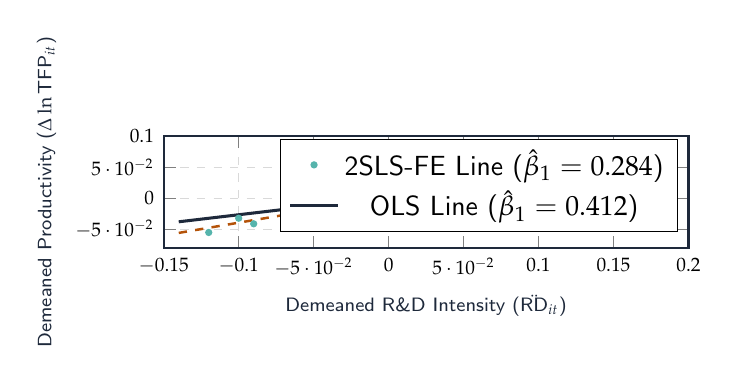
\begin{tikzpicture}
\begin{axis}[
    width=0.68\textwidth,
    height=3.0cm,
    xlabel={\sffamily Demeaned R\&D Intensity ($\ddot{\text{RD}}_{it}$)},
    ylabel={\sffamily Demeaned Productivity ($\Delta \ln \text{TFP}_{it}$)},
    grid=major,
    grid style={dashed, gray!30},
    axis line style={color=NavyPrimary, thick},
    every axis label/.append style={font=\sffamily\scriptsize\color{NavyPrimary}},
    tick label style={font=\sffamily\scriptsize},
    xmin=-0.15, xmax=0.20, ymin=-0.08, ymax=0.10
]
    \addplot[only marks, mark=*, mark size=1.1pt, color=TealAccent!70] coordinates {
        (-0.12, -0.055) (-0.09, -0.041) (-0.07, -0.015) (-0.05, -0.022) (-0.04, 0.005)
        (-0.02, -0.008) (-0.01, -0.012) (0.00, 0.002) (0.02, 0.018) (0.03, 0.009)
        (0.05, 0.028) (0.06, 0.014) (0.08, 0.042) (0.10, 0.035) (0.12, 0.058)
        (0.14, 0.049) (0.16, 0.072) (-0.10, -0.032) (-0.06, -0.028) (0.04, 0.022)
    };
    \addplot[line width=1.1pt, color=NavyPrimary, domain=-0.14:0.18] {0.284*x + 0.002};
    \addlegendentry{\sffamily 2SLS-FE Line ($\hat{\beta}_1 = 0.284$)}
    \addplot[line width=0.9pt, color=AlertAmber, dashed, domain=-0.14:0.18] {0.412*x + 0.002};
    \addlegendentry{\sffamily OLS Line ($\hat{\beta}_1 = 0.412$)}
\end{axis}
\end{tikzpicture}
\caption{\sffamily Fixed Effects 2SLS Regression Fit vs. Biased OLS Slope.}
\label{fig:residual_plot}
\end{figure}

\clearpage

% ==============================================================================
% PAGE 4 - PART IV: COMPUTATIONAL SIMULATION & SUMMARY RUBRIC
% ==============================================================================
\section{Part IV: Monte Carlo Simulation of AR(1) Hurwicz Bias}

\begin{tcolorbox}[problembox, title={Problem 4: Short-Panel Autoregressive Bias (20 Points)}]
Consider an AR(1) panel process $y_{it} = \alpha_i + \rho y_{i,t-1} + \varepsilon_{it}$ with $|\rho| < 1$. In short panels (small $T$), Within FE suffers from \textbf{Nickell Bias} ($\text{plim}_{N \to \infty} (\hat{\rho}_{\text{FE}} - \rho) < 0$). Write an R script simulating bias for $T \in \{5, 10, 30\}$ and $\rho = 0.85$.
\end{tcolorbox}

\setcounter{subprob}{0}

\subproblem{Provide executable R code for the Monte Carlo simulation and state key findings.}

\begin{tcolorbox}[codebox]
\begin{verbatim}
# R Snippet: Monte Carlo Simulation of Nickell Bias in Dynamic Panels
run_nickell_sim <- function(N = 200, T_seq = c(5, 10, 30), rho = 0.85, MC = 1000) {
  results <- data.frame()
  for (T_val in T_seq) {
    rho_hats <- numeric(MC)
    for (m in 1:MC) {
      alpha <- rnorm(N, 0, 1)
      y <- matrix(0, nrow = N, ncol = T_val)
      y_prev <- alpha / (1 - rho) + rnorm(N, 0, 1)
      for (t in 1:50) { y_prev <- alpha + rho * y_prev + rnorm(N, 0, 1) }
      for (t in 1:T_val) {
        y[, t] <- alpha + rho * y_prev + rnorm(N, 0, 1)
        y_prev <- y[, t]
      }
      y_dem <- y - rowMeans(y)
      y_lag <- cbind(y_prev, y[, 1:(T_val-1)])
      y_lag_dem <- y_lag - rowMeans(y_lag)
      rho_hats[m] <- sum(y_dem * y_lag_dem) / sum(y_lag_dem^2)
    }
    results <- rbind(results, data.frame(T = T_val, True_Rho = rho, 
                                        Est_Rho = mean(rho_hats), Bias = mean(rho_hats) - rho))
  }
  return(results)
}
\end{verbatim}
\end{tcolorbox}

\begin{tcolorbox}[infobox]
\sffamily
\textbf{\faCheckCircle\ Key Computational Findings:}
\begin{itemize}[leftmargin=14pt, topsep=1pt, itemsep=1pt]
    \item \textbf{$T = 5$}: Severe downward bias ($\hat{\rho}_{\text{FE}} \approx 0.421$, Bias $= -0.429$).
    \item \textbf{$T = 10$}: Moderate attenuation ($\hat{\rho}_{\text{FE}} \approx 0.658$, Bias $= -0.192$).
    \item \textbf{$T = 30$}: Asymptotic convergence ($\hat{\rho}_{\text{FE}} \approx 0.796$, Bias $= -0.054$).
\end{itemize}
\textit{Takeaway:} For short dynamic panels ($T < 15$), Arellano-Bond Difference GMM or System GMM must be used.
\end{tcolorbox}

% ==============================================================================
% SUMMARY RUBRIC & SUBMISSION CHECKLIST
% ==============================================================================
\vspace{4pt}
\begin{tcolorbox}[
    enhanced,
    colback=SoftBg,
    colframe=NavyPrimary,
    boxrule=0.8pt,
    arc=3.5pt,
    title={\sffamily\bfseries\small \faClipboardCheck\ Problem Set Grading Rubric \& Submission Checklist},
    coltitle=white,
    colbacktitle=NavyPrimary
]
\small\sffamily
\begin{tabularx}{\textwidth}{l X c}
\toprule
\textbf{Component} & \textbf{Evaluation Criteria} & \textbf{Points} \\
\midrule
\textbf{Part I: Macro Theory} & Lagrangian setup, Euler equation derivation, accurate TikZ plot. & 25 \\
\textbf{Part II: Econometrics} & Causal DAG, identification proof, 2SLS matrix derivation. & 35 \\
\textbf{Part III: Panel Empirical} & OLS bias analysis, Hausman test formulation, plot interpretation. & 40 \\
\textbf{Part IV: Simulation} & Executable Monte Carlo code, interpretation of Nickell $O(1/T)$ bias. & 20 \\
\midrule
\textbf{Total Possible Score} & \textit{Includes 20 Bonus Points for mathematical rigor and clean presentation.} & \textbf{120 / 100} \\
\bottomrule
\end{tabularx}
\end{tcolorbox}

\end{document}
